\documentclass[a4paper,12pt]{article}
\usepackage[utf8]{inputenc}
\usepackage{graphicx}
\graphicspath{ {./imgs/} }
\usepackage{fancyhdr}
\usepackage{geometry}
\usepackage{hyperref}
\usepackage{longtable}
\usepackage{array}
\usepackage{booktabs}
\usepackage{caption}
\usepackage{amsmath}

% Adjust margins
\geometry{
    top=4cm,
    bottom=2.5cm,
    left=2.5cm,
    right=2.5cm,
    headheight=3cm,
    headsep=0.5cm,
    }

\fancypagestyle{firstpage}{
    \fancyhf{}
    \fancyhead[L]{
\includegraphics[height=1.5cm]{heig_logo.png}}
    \fancyhead[R]{
\includegraphics[height=1.5cm]{reds_logo.png}}
    \fancyfoot{}
}

\fancypagestyle{otherpages}{
    \fancyhf{}
    \fancyhead[L]{
\includegraphics[height=1.5cm]{heig_logo.png}}
    \fancyhead[R]{%
        \small Laboratoire 2: Roofline \\
        Urs Behrmann \\
    }
    \fancyfoot[C]{\small page \thepage}
}

\author{Urs Behrmann}
\setlength{\parskip}{1em}
\setlength{\parindent}{0pt}
\renewcommand{\arraystretch}{1.4}

\begin{document}

\emergencystretch=1em
\thispagestyle{firstpage}

\vspace*{2cm}
\begin{center}
    \Huge Laboratoire 2 \\
    \vspace{0.2cm}
    \Large Roofline\\
    \vspace{1cm}
    \small Départements : TIC\\
    Unité d'enseignement HPC\\
\end{center}

\vspace{9cm}

\begin{flushleft}
    \begin{tabular}{@{}l l@{}}
        \textbf{Auteurs :}       & \textbf{Urs Behrmann} \\
        \textbf{Professeur :}    & \textbf{Alberto Dassatti} \\
        \textbf{Assistant :}     & \textbf{Bruno Da Rocha Carvalho} \\
        \textbf{Classe :}        & \textbf{HPC} \\
        \textbf{Salle de labo :} & \textbf{A09} \\
        \textbf{Date :}          & \textbf{23.03.2026} \\
    \end{tabular}
\end{flushleft}

\newpage
\pagestyle{otherpages}
\tableofcontents
\newpage

% ─────────────────────────────────────────────────────────────────
\section{Roofline de la machine}

\subsection{Architecture CPU}

Les mesures ont été faites sur un \textbf{AMD Ryzen 7 5800H} (architecture Zen3),
avec 8 cœurs physiques (16 threads) et 16~MB de cache L3.
Tout est en mono-thread (core 2), en double précision, compilé sans optimisation (\texttt{-O0}).

\subsection{Plafonds mesurés}

On a mesuré les deux paramètres du Roofline avec \texttt{likwid-bench}~:

\begin{verbatim}
$ likwid-bench -t peakflops -W N:30kB:1
...
MFlops/s:   10712.35
MByte/s:    5356.17
\end{verbatim}

\begin{verbatim}
$ likwid-bench -t load -W N:2GB:1
...
MByte/s:    26040.92
\end{verbatim}

\begin{center}
\begin{tabular}{lrp{7cm}}
    \toprule
    \textbf{Paramètre} & \textbf{Valeur} & \textbf{Commande} \\
    \midrule
    Calcul max (\textit{maxperf})
        & 10\,712.35 MFlops/s
        & \texttt{likwid-bench -t peakflops -W N:30kB:1} \\
    Bande passante max (\textit{maxband})
        & 26\,040.92 MB/s
        & \texttt{likwid-bench -t load -W N:2GB:1} \\
    \bottomrule
\end{tabular}
\end{center}

Le \textit{knee} (point de transition) est à
$AI = \frac{10712.35}{26040.92} \approx \mathbf{0.411}$~FLOP/Byte.
En dessous de cette valeur le kernel est limité par la mémoire, au-dessus il est limité par le calcul.

\newpage

\subsection{Graphique Roofline}

\begin{figure}[h!]
    \centering
    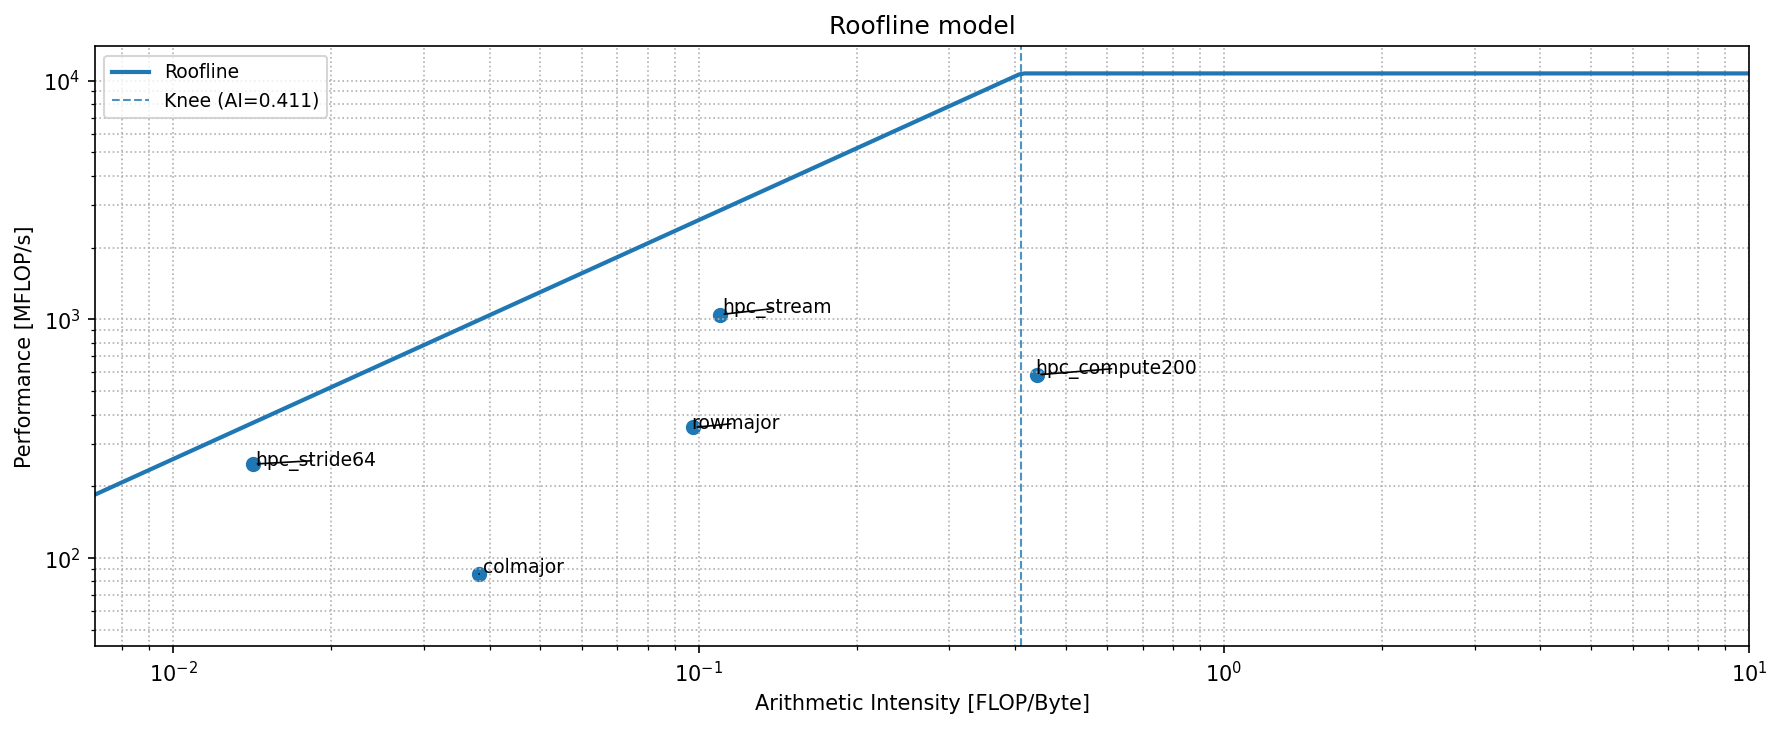
\includegraphics[width=\textwidth]{roofline.png}
    \caption{Roofline — AMD Ryzen 7 5800H, mono-thread, double précision scalaire, \texttt{-O0}.
             Tous les points sont sous le plafond théorique.}
    \label{fig:roofline}
\end{figure}

\newpage

% ─────────────────────────────────────────────────────────────────
\section{Mesures des cas d'étude}

Les mesures ont été obtenues avec \texttt{likwid-perfctr} (groupe \texttt{HPC}, core 2,
\texttt{sudo}) en utilisant les marqueurs LIKWID intégrés dans le code. Les valeurs AI et
Perf proviennent directement des compteurs matériels du processeur.

\begin{verbatim}
sudo likwid-perfctr -C 2 -g HPC -m ./roofline_demo hpc_stream 50000000
\end{verbatim}

\begin{center}
\begin{tabular}{lrrl}
    \toprule
    \textbf{Cas d'étude} & \textbf{AI [FLOP/Byte]} & \textbf{Perf [MFlops/s]} & \textbf{Paramètres} \\
    \midrule
    \texttt{hpc\_stream}         & 0.1099 & 1048 & \texttt{n=50\,000\,000} \\
    \texttt{hpc\_stride64}       & 0.0142 &  248 & \texttt{n=50M, stride=64} \\
    \texttt{hpc\_compute200}     & 0.4406 &  586 & \texttt{n=1M, iters=200} \\
    \texttt{rowmajor}            & 0.0976 &  353 & \texttt{N=4096} \\
    \texttt{colmajor}            & 0.0382 &   86 & \texttt{N=4096} \\
    \bottomrule
\end{tabular}
\captionof{table}{Résultats des 4 cas d'étude — mesurés par compteurs matériels LIKWID.}
\end{center}

\textbf{Écart entre AI théorique et AI mesurée.}

L'AI analytique suppose que seules les données utiles transitent par la DRAM. En réalité,
plusieurs effets matériels augmentent le trafic réel~:
\begin{itemize}
    \item \textit{Write-allocate}~: avant d'écrire une ligne de cache, le processeur la charge
    d'abord depuis la DRAM, ce qui double le trafic pour les écritures.
    \item \textit{Granularité des lignes de cache}~: avec \texttt{hpc\_stride64}, chaque accès
    charge 64 octets mais n'en utilise que 8 (12.5\% d'efficacité), ce qui fait exploser le
    trafic DRAM réel et effondre l'AI mesurée de 0.188 à 0.014.
    \item \textit{Réutilisation du cache}~: pour \texttt{hpc\_compute200}, les données tiennent
    en cache après le premier chargement. Le trafic DRAM est donc minime, ce qui donne une AI
    mesurée de 0.44 — très différente de l'AI théorique de 75.25.
\end{itemize}

\newpage

% ─────────────────────────────────────────────────────────────────
\section{Analyse comparative}

\subsection{stream vs stride — memory coalescing}

\texttt{hpc\_stream} et \texttt{hpc\_stride64} ont la même AI théorique, mais les compteurs
LIKWID révèlent une réalité très différente~: AI=0.110 et 1048~MFlops/s pour \texttt{stream},
contre AI=0.014 et 248~MFlops/s pour \texttt{stride64}.

C'est un problème de \textbf{memory coalescing} (concept vu en CNM). Une ligne de cache
fait 64~octets, soit 8 \texttt{double}. Quand les accès sont contigus (\texttt{stream},
stride=1), chaque ligne chargée est utilisée à 100\%~: on profite pleinement des 8 valeurs
ramenées depuis la DRAM. C'est du bon coalescing.

Avec un stride de 64, chaque itération saute directement à la prochaine ligne de cache~:
on charge 64 octets mais on n'utilise qu'un seul \texttt{double} (8 octets), soit un rendement
de 12.5\%. LIKWID mesure 10.5~GB de trafic DRAM pour seulement 150M FLOPs — le trafic
mémoire est ~8× ce que l'analyse théorique prédit. C'est exactement ce qu'on cherche à
éviter avec le coalescing~: regrouper les accès pour charger chaque ligne une seule fois
et l'utiliser entièrement.

\subsection{stream vs compute — mémoire vs calcul}

\texttt{hpc\_stream} ($AI = 0.110$ mesuré, sous le \textit{knee} à 0.411) est limité par la
bande passante mémoire. Sa performance de 1048~MFlops/s est bien en dessous du plafond de
calcul (10\,712~MFlops/s), mais c'est normal~: il n'y a pas assez d'opérations par octet
transféré pour occuper le processeur.

\texttt{hpc\_compute200} ($AI = 0.44$ mesuré) est un cas très intéressant~: son AI se
situe juste au-dessus du \textit{knee} (0.411), donc à la frontière entre mémoire et
calcul. Sa performance de 586~MFlops/s reste loin du plafond de 10\,712~MFlops/s à cause
du \texttt{-O0}~: sans vectorisation, le processeur ne fait qu'une opération scalaire à la
fois alors qu'il pourrait en faire 4 en parallèle avec AVX2. L'AI théorique était 75.25,
mais en pratique les données tiennent en cache — le vrai goulot d'étranglement est le calcul
scalaire, pas la DRAM.

\subsection{rowmajor vs colmajor — localité spatiale et coalescing}

Ces deux kernels ont la même AI théorique, mais LIKWID révèle des valeurs très différentes~:
\texttt{rowmajor} (AI=0.098, 353~MFlops/s) est 4.1× plus rapide que \texttt{colmajor}
(AI=0.038, 86~MFlops/s).

En C, les tableaux 2D sont stockés ligne par ligne (\textit{row-major}).
\texttt{rowmajor} parcourt les éléments dans l'ordre où ils sont en mémoire, donc les accès
sont coalescés~: chaque ligne de cache chargée contient les 8 prochains éléments à utiliser.

\texttt{colmajor} fait le contraire~: il saute de ligne en ligne, soit 4096 éléments
($4096 \times 8 = 32$~kB) entre deux accès consécutifs. Résultat~: quasiment aucun réemploi
de ligne de cache, les accès ne sont pas coalescés, et on se retrouve à faire autant de
cache-misses que d'éléments lus.

\newpage

% ─────────────────────────────────────────────────────────────────
\section{Propositions d'amélioration théoriques}

\subsection{hpc\_stride — tuilage (blocking)}

Avec \texttt{stride=64}, chaque accès tombe dans une nouvelle ligne de cache et les
7 autres \texttt{double} chargés avec elle ne sont jamais utilisés.

L'idée du \textit{tuilage} est de découper le tableau en petits blocs de taille $B$ qui
tiennent entièrement dans le cache L1 (32~kB sur Zen3). On traite un bloc entier avant de
passer au suivant, ce qui force la réutilisation de chaque ligne de cache chargée.
Au lieu d'accéder à \texttt{x[0]}, \texttt{x[64]}, \texttt{x[128]}..., on traiterait
d'abord tous les éléments du bloc \texttt{x[0..B]}, puis \texttt{x[B..2B]}, etc.

\subsection{hpc\_compute — déroulage de boucle}

Dans \texttt{heavy\_work}, chaque itération dépend du résultat de la précédente
(\textit{dépendance de données}). Le processeur doit donc attendre la fin de chaque
itération avant de commencer la suivante, même s'il pourrait en traiter plusieurs à la fois.

En déroulant la boucle (\textit{loop unrolling}), on traite 4 éléments de \texttt{x}
à la fois, chacun avec ses propres variables de calcul. Ces 4 chaînes sont indépendantes
entre elles, donc le processeur peut les exécuter en parallèle et mieux occuper ses
unités arithmétiques.

\subsection{colmajor — tuilage 2D}

L'accès colonne par colonne saute de $N \times 8 = 32$~kB entre deux itérations
consécutives (pour N=4096), soit 512 lignes de cache. Chaque accès est un cache-miss.

Avec un tuilage $B \times B$ (avec $B$ choisi pour que le bloc tienne dans le cache L1),
on réorganise les boucles pour travailler sur un petit bloc à la fois. Les lignes de cache
chargées pour les premières itérations du bloc sont encore en cache pour les suivantes,
ce qui réduit drastiquement le nombre de cache-misses.

\end{document}
